% =====================================================================
% Narrative attractors in a shared-world RPG played by language-model agents
% Target: The International Journal of Games and Social Impact (IJGSI),
%         Vol. 5, No. 4 -- Games, Gamification, Media Literacy and
%         Transformation in Educational Contexts.
% Anonymised manuscript for double-blind review. Author data go in
% titlepage.tex (separate file). References: APA 7 via biblatex-apa.
% Compile in Overleaf with the "biber" backend (Menu > Settings > Compiler
% pdfLaTeX; the bibliography tool is chosen automatically by latexmk).
% =====================================================================
\documentclass[12pt]{article}

\usepackage[utf8]{inputenc}
\usepackage[T1]{fontenc}
\usepackage[english]{babel}
\usepackage{csquotes}
\usepackage{mathptmx}                      % Times, as the journal asks
\usepackage[a4paper,margin=2.54cm]{geometry}
\usepackage{setspace}\onehalfspacing
\usepackage{graphicx}
\usepackage{booktabs}
\usepackage{tabularx}
\usepackage{fancyhdr}
\usepackage{xcolor}
\usepackage[hidelinks]{hyperref}
\usepackage[style=apa,backend=biber]{biblatex}
\addbibresource{referencias.bib}

\graphicspath{{figuras/}}

% page number top right, as required
\pagestyle{fancy}\fancyhf{}\fancyhead[R]{\thepage}
\renewcommand{\headrulewidth}{0pt}

% the generated stories are in Portuguese; quotes are translated
\newcommand{\pt}[1]{\textit{#1}}

\title{\textbf{\textit{NARRATIVE ATTRACTORS: WHY STORIES CONVERGE IN A SHARED-WORLD ROLE-PLAYING GAME PLAYED BY LANGUAGE-MODEL AGENTS}}}
\author{[Anonymised for review]}
\date{}

\begin{document}
\maketitle
\thispagestyle{fancy}

\begin{abstract}
\noindent
Generative AI is entering classrooms as a co-author of stories and as a game
master for role-playing games. We ask whether a shared fictional world, in
which several language-model agents act freely with no plot structure
imposed on them, produces many storylines that open and close or collapses
into a single story. Using a pre-registered instrument that records every
event and its declared causes, we built the causal graph of 44 simulated
sessions (3,744 events, four versioned models, two worlds). Storylines
disappear mostly by fusion, not by closure: 64\% of them are absorbed into
another storyline and fewer than 5\% reach a stable ending. Almost all storylines
are born on the second day, and in 36 of 44 sessions a single storyline
remains, typically by day five. Convergence is driven first by density
(almost every event cites a cause), and its course is shaped by attractors:
the first fusions join characters whose premises already referred to each
other (75\% against 61\% under a density-preserving null model) and happen
in the places those premises name. We discuss what this means for critical
AI literacy and for the design of educational role-play with generative
agents.
\end{abstract}

\noindent\textit{Keywords: generative AI; role-playing games; emergent narrative; causal graphs; attractors; AI literacy; media literacy}

% ---------------------------------------------------------------------
\section{Introduction}
% ---------------------------------------------------------------------

Tabletop role-playing games have long been used in education as spaces for
shared imagination, perspective-taking and collaborative problem solving
\parencite{fine1983,bowman2010,daniau2016}. Their narrative is not written in
advance: it emerges from what the participants do inside a shared world,
under explicit and implicit rules \parencite{montola2008}. Large language
models (LLMs) now make it possible to populate such worlds with artificial
characters that remember, plan and talk to each other
\parencite{park2023}, and to place an AI in the role of the game master
\parencite{callisonburch2022}. Teachers and students are already
experimenting with these uses.

At the same time, a growing body of evidence shows that generative models
homogenise what they help to produce. Writers assisted by a model produce
less diverse texts \parencite{padmakumar2024}; stories written with AI ideas
are individually rated as more creative but are more similar to each other
\parencite{doshi2024}; LLM stories reuse a narrow repertoire of plot elements
\parencite{xu2025} and follow more uniform arcs than human stories
\parencite{tian2024,begus2024}. These studies look at single texts produced
from a prompt. Much less is known about what happens to the
\emph{structure} of a story when it is not written by one model in one pass
but emerges, day after day, from the actions of several agents in a shared
world, the situation closest to a role-playing game.

This paper reports an experiment on that question. We built a simulator in
which language-model agents live in a small fictional town, each with an
objective, a secret and a few beliefs, and act freely for 12 to 20 in-game
days. Nothing in the prompts mentions acts, climax, resolution or any other
narrative structure. Every action is recorded as an event, together with the
earlier events the agent declares as its causes. The result is a causal graph
in which a storyline can be read as a connected set of events
\parencite{trabasso1985}. Our pre-registered hypothesis was that such a free
story converges: storylines that emerge tend to close, and beginning, middle
and end appear as properties of the graph rather than as phases imposed on
the generation.

The answer we found is more specific, and more relevant for education, than
a simple yes or no. Storylines do converge, but almost never by closing:
they \emph{merge} until a single story remains. We describe that process in
the vocabulary of dynamical systems, where an \emph{attractor} is a state, or
set of states, toward which trajectories starting from many different
initial conditions evolve \parencite{strogatz2015,lorenz1963}. We show that
the single-story state behaves as a global attractor of these simulated
worlds, and we identify the \emph{attractor events} that pull separate
storylines together: events in which characters whose premises were already
entangled meet, in the places those premises name.

The contributions are threefold. First, an auditable method to measure
convergence in emergent narratives that separates two processes usually
confounded, the closure of a storyline and its fusion with another. Second,
empirical evidence, from 44 sessions with four versioned models, that fusion
dominates and that its course is shaped by the initial conditions authored
by humans. Third, a discussion of what this means for critical AI literacy:
when generative agents tell stories together, the story that emerges is
less open than it looks, and the levers that shape it are visible and can be
taught.

% ---------------------------------------------------------------------
\section{Background}
% ---------------------------------------------------------------------

\subsection{Stories as causal graphs}

Structuralist narratology distinguishes the events that hold a plot
together, \emph{kernels} or \emph{nuclei}, from those that elaborate it,
\emph{satellites} or \emph{catalysers}
\parencite{barthes1975,chatman1978}. Cognitive studies of comprehension
operationalised this idea as a causal network: an event belongs to the main
chain of a story when it has causal antecedents and consequences, and
readers remember and judge as important the events with more causal
connections \parencite{trabasso1985}. Computational narrative inherited the
representation. Narrative planners build plots as partially ordered causal
structures \parencite{riedl2010}, and simulation-driven storytelling treats
the log of a simulated world as raw material from which stories are later
\emph{curated} \parencite{ryan2018}. We follow this tradition: each event
records its declared causes, and a storyline is a connected component of the
resulting graph.

\subsection{Emergent narrative and shared worlds}

Emergent narrative is the idea that a story can arise from the interaction
of autonomous characters and participants rather than from a script
\parencite{aylett1999,louchart2004}. Its persistent difficulty is
\emph{shape}: autonomous agents produce events, but events do not
necessarily add up to stories with beginnings and endings
\parencite{riedl2013}. Interactive drama addressed the problem with a drama
manager that steers the action toward a planned arc \parencite{mateas2003};
storylet systems address it by authoring small, conditioned narrative
fragments \parencite{kreminski2018}. Game studies add a spatial perspective:
game worlds tell stories through the arrangement of places, which channel
movement and encounters \parencite{jenkins2004}. Role-playing studies, in
turn, show that the rules that shape a shared fiction are often invisible
and social rather than written \parencite{montola2008,fine1983}.

Generative agents change the terms of this debate. Their behaviour is
believable and memory-driven \parencite{park2023}, but it is produced by a
model trained to continue text coherently, which may favour connecting new
events to existing ones over starting new threads. Whether that tendency
yields well-shaped stories, endless sprawl or something else is an empirical
question.

\subsection{Attractors}

In a dynamical system, an attractor is a set of states toward which the
system evolves from a wide range of initial conditions; the set of initial
conditions that lead to it is its \emph{basin of attraction}
\parencite{strogatz2015}. Chaotic systems combine sensitivity to initial
conditions at the level of individual trajectories with stable large-scale
structure: two trajectories of the Lorenz system diverge quickly, yet both
remain on the same attractor \parencite{lorenz1963}. We use the concept in
two ways. At the macro level, we ask whether different sessions, with
different models, worlds, seeds and conditions, end in the same structural
state. At the micro level, we call \emph{attractor events} the events
through which separate storylines are pulled into one, directly (an event
that cites causes in both storylines) or indirectly (through intermediate
events), and we ask what they have in common. The analogy is heuristic: a
simulated story is not a low-dimensional deterministic system. But it gives
precise questions: what is the end state, how fast is it reached, how large
is its basin, and which initial conditions decide the path.

\subsection{AI literacy and media literacy}

Media literacy asks learners to analyse how messages are constructed and by
whom \parencite{hobbs2010}. AI literacy extends the question to systems that
generate content: learners should understand what AI can and cannot do, how
it represents knowledge and how its outputs are shaped
\parencite{long2020,unesco2024}. Homogenisation findings
\parencite{doshi2024,xu2025} have made the shaping of generated stories a
topic in its own right. Most work, however, considers a single generated
text. Shared-world play with AI agents is a different object: the story is
co-produced over time by many prompts, and the forces that shape it are
distributed across the world design, the agents and the rules of play. Making
those forces visible is a precondition for using such play critically in
education.

% ---------------------------------------------------------------------
\section{Method}
% ---------------------------------------------------------------------

\subsection{The simulator}

The simulator runs a small fictional town for a fixed number of in-game
days. Each world defines five or six places, three factions and a
cast of agents, each with an objective, a secret and two beliefs
(Table~\ref{tab:mundos}). We used two worlds written for the study:
\emph{Porto das Brumas}, a harbour town where salt merchants, a smuggling
brotherhood and the harbour guard compete, and \emph{Vale Silente}, a
mountain village isolated by a landslide before winter. Sessions used six
agents. Every day, one call to the agents' model decides what each character
does; for each action, the model writes a short text, names the place and
the witnesses, and lists the identifiers of the recent events (from the
previous three days) that made the action possible. The prompt explicitly
allows the list to be empty. A second call writes what characters tell
each other. A fixed \emph{curator} model narrates storylines that become
stable, and a fixed synthetic player can take part in some conditions.
The model of the agents is the experimental variable; the curator and the
player are held constant across conditions.

\begin{table}[t]
\centering\small
\caption{The two worlds and the premises of their six active agents (abridged; translated).}
\label{tab:mundos}
\begin{tabularx}{\textwidth}{@{}p{2.2cm}X@{}}
\toprule
World & Agents (objective; secret or belief that refers to another agent) \\
\midrule
Porto das Brumas &
Odete, merchant (wants the late Vasco's warehouse; owes money to the smuggling brotherhood) ·
Brás, guard captain (takes bribes; believes the new inspector is spying on him) ·
Lia, smuggler (wants to lead the brotherhood; informs the guard) ·
Tomás, chaplain (knows who was in the warehouse the night Vasco died) ·
Iracema, Vasco's widow (believes her husband hid papers in the warehouse) ·
Nuno, customs inspector (investigates why the customs books do not add up) \\
\addlinespace
Vale Silente &
Anselmo, elder (secretly sold the village's grain) ·
Marta, shepherd (blames wolves for losses she caused) ·
Sister Clara (believes the miller hides something) ·
Joaquim, miller (shelters a wounded stranger in the mill) ·
Benedita (wants to open a trail before winter) ·
Rui, goatherd (saw someone leaving the mill at dawn) \\
\bottomrule
\end{tabularx}
\end{table}

Nothing in any prompt refers to narrative structure. An automated test
scans every prompt for structural terms (act, phase, climax, resolution,
hero's journey and their Portuguese equivalents) and for instructions to
converge (tie up, conclude, resolve, close), and fails the build if any is
present. As a control, the simulator also runs a conventional
three-act game master over the same worlds.

\subsection{From events to storylines}

Each session yields an event log and a directed graph whose edges go from a
declared cause to its effect. Following the causal-network view of
narrative \parencite{trabasso1985}, a \emph{storyline} is a connected
component of the graph of events with causal connections, recomputed every
day. A storyline is \emph{stable} when it receives no new consequence for
$k = 3$ consecutive days.

Our pre-registration defined convergence through the number of open
storylines, which should stop growing in the last third of the session
\parencite{nosek2018}. A first round of validation showed that this measure
was confounded: the number of open storylines fell in almost every session,
but mostly because storylines merged, not because they ended. We therefore
amended the pre-registration, before any confirmatory campaign, to track the
\emph{lineage} of each storyline: its \emph{birth} (a component whose events
belonged to no storyline the day before), its \emph{fusion} (its events
become part of another storyline) and its \emph{closure by stability}. The
main metric became the share of storylines that close by stability before
being absorbed. All amendments are dated and public in the repository.

Formally, let $G_d = (V_d, E_d)$ be the causal graph at the end of day $d$,
where $V_d$ holds the events of days $1,\dots,d$ and $(u, v) \in E_d$ when
event $v$ declares $u$ as a cause and $u$ is not later than $v$. Let
$\mathcal{T}_d$ be the set of connected components of the subgraph of events
that have at least one causal connection. A storyline $T \in \mathcal{T}_d$
is \emph{born} on day $d$ if none of its events belonged to a storyline in
$\mathcal{T}_{d-1}$; it \emph{fuses} on day $d$ if its events belong, on day
$d$, to a storyline with a different identifier; and it \emph{closes} on day
$d$ if it is stable on day $d$ for the first time. A storyline that keeps its
events but receives a new identifier because of a fusion is a
\emph{renaming}, not a birth. If $N$ storylines are born in a session, $C$ of
them close before fusing and $F$ fuse before closing, the main metric is
$C/N$ and its companion is $F/N$. Because components only grow or merge as
events are added, $\mathcal{T}_d$ can only lose members by fusion or gain
them by birth; closure does not remove a storyline from the graph, it only
marks it as having stopped growing. The number of open storylines falls by
one both when a storyline closes and when two of them merge, which is why
that number alone cannot distinguish an ending from a merger.

\subsection{Sessions}

We analyse 44 sessions of the shared world, generated with four versioned
models as agents (\texttt{claude-haiku-4-5-20251001},
\texttt{claude-sonnet-4-6}, \texttt{claude-sonnet-5} and
\texttt{claude-opus-5}), in four rounds:
(1) 16 sessions of 12 days, crossing the four models, the two worlds and
whether the state of storylines is shown to the agents;
(2) 8 sessions in which each cause carries a declared type and strength;
(3) 8 sessions in which agents may cite at most two causes per action; and
(4) 12 sessions of 20 days, with two models, two worlds and three
repetitions with new seeds. Rounds 2 and 3 use the same models, worlds and
seeds as the corresponding sessions of round 1. Eight sessions of the
three-act control serve as a reference. In total, the shared-world sessions
contain 3,744 events.

\subsection{Validation of the declared causes}

A causal graph built from what a model declares is only as good as those
declarations. We validated them in three ways. A blind judge model, not used
as a generator, rated declared links as plausible far more often than
distractor pairs from the same session (97\% against 73\%). In a counterfactual test, a judge
estimated how necessary event $A$ was for event $B$ on a 0--100 scale: 67 on
average for declared direct links, 44 for indirect ancestors and 21 for
unlinked pairs, with an area under the ROC curve of 0.92 between direct and
unlinked pairs. Finally, a null model rewired every event's causes at random
among earlier events, keeping how many causes each event has, and the
analysis was repeated 500 times per session. Human annotation of a stratified
sample of 216 links by two annotators has been prepared and is reported
separately.

\subsection{Measuring attractors}

We use four measures. The \emph{basin} is the number of storylines not yet
absorbed on each day, and the day on which a single storyline remains.
\emph{Direct fusions} are those in which the event that merges two
storylines cites causes in both of them; the others are indirect.
\emph{Premise attraction} compares, for the first fusion between two
storylines that had not merged before, whether the characters who started
them are linked in the world premises. Two characters are linked when the
objective, secret or a belief of one of them mentions the other by name,
title or unique role, or something only the other owns
(Table~\ref{tab:mundos}); the coding is published with the analysis
script. The comparison is made against the same pairs under the null model,
so that the effect of link density is discounted. \emph{Spatial attraction}
compares the share of fusion events that happen in the places named in more
than one premise (the warehouse and the customs house in Porto das Brumas;
the mill in Vale Silente) with the same share under the null model. We also
measure the entropy of the distribution of events over places on each day,
and the concentration of incoming links, to check whether a few events act
as hubs \parencite{barabasi1999,newman2018}. All analyses are scripted and
reproducible from the event logs.

% ---------------------------------------------------------------------
\section{Results}
% ---------------------------------------------------------------------

\subsection{Storylines merge; they rarely close}

Figure~\ref{fig:fusao} shows what happens to the storylines of the 32
twelve-day sessions. By day 12, 64\% of them have been absorbed by another
storyline, and only 4.5\% have reached a stable ending. In the first round
alone (16 sessions), 59\% of the storylines were absorbed and 8\% closed;
only 2 of the 16 sessions (12.5\%) satisfy the amended definition of
convergence, whereas 15 of 16 (94\%) satisfied the original one. The
original measure would have confirmed the hypothesis by an artefact.

\begin{figure}[t]
\centering
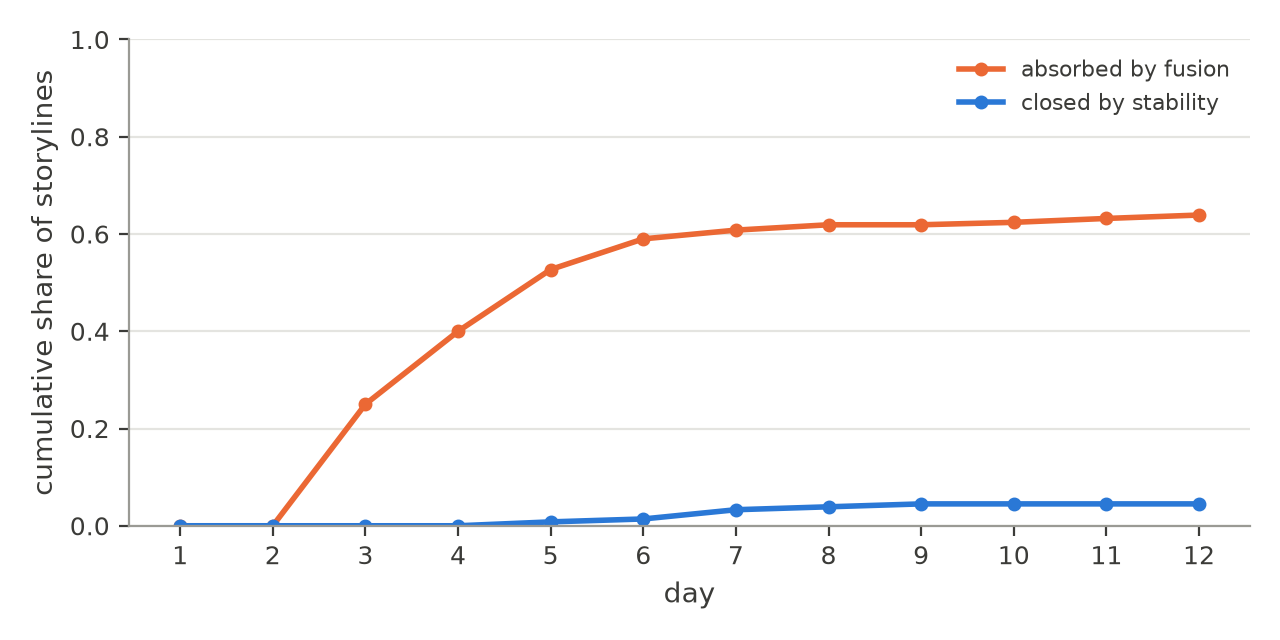
\includegraphics[width=0.78\textwidth]{fusao_fechamento.png}
\caption{Cumulative share of storylines absorbed by fusion and closed by
stability, mean of the 32 twelve-day shared-world sessions.}
\label{fig:fusao}
\end{figure}

\subsection{A single-story attractor}

Across the 44 sessions, 191 of the 194 storylines were born on the second
day, when the first actions start citing each other. After that, new
storylines practically never appear: of the 3,480 events generated
after the first day, only 9 (0.3\%) cite no cause, although the prompt says
that the list may be empty. Each event cites 1.95 causes on average. An
event with a cause always joins an existing storyline, so the world's initial
storylines are the only ones it will ever have.

The storylines then merge quickly (Figure~\ref{fig:bacia}). Half of all
fusions happen by day 4, and 81\% by day 5. In 37 of the 44 sessions a
single unabsorbed storyline remains at some point, at a median of day 5
(interquartile range 4--7), and 36 sessions end that way. Twenty-day
sessions do not reopen the story: the curve keeps approaching one. In 11 of
the 12 twenty-day sessions a single unabsorbed storyline remained at the
end (in the twelfth, one storyline closed and another absorbed the rest), and
in ten of them the last fusion happened by day 7. The end state is the same across the four models, both
worlds, both levels of information about the storylines, and every
intervention we tried: asking for the type and strength of each cause made
agents cite more causes (1.71 to 2.30 per event in paired sessions) and
removed all closures; limiting causes to two per action barely reduced the
density (1.71 to 1.57) and did not reduce fusion. The single-story state
behaves as a global attractor, with a basin that covers every condition we
sampled.

\begin{figure}[t]
\centering
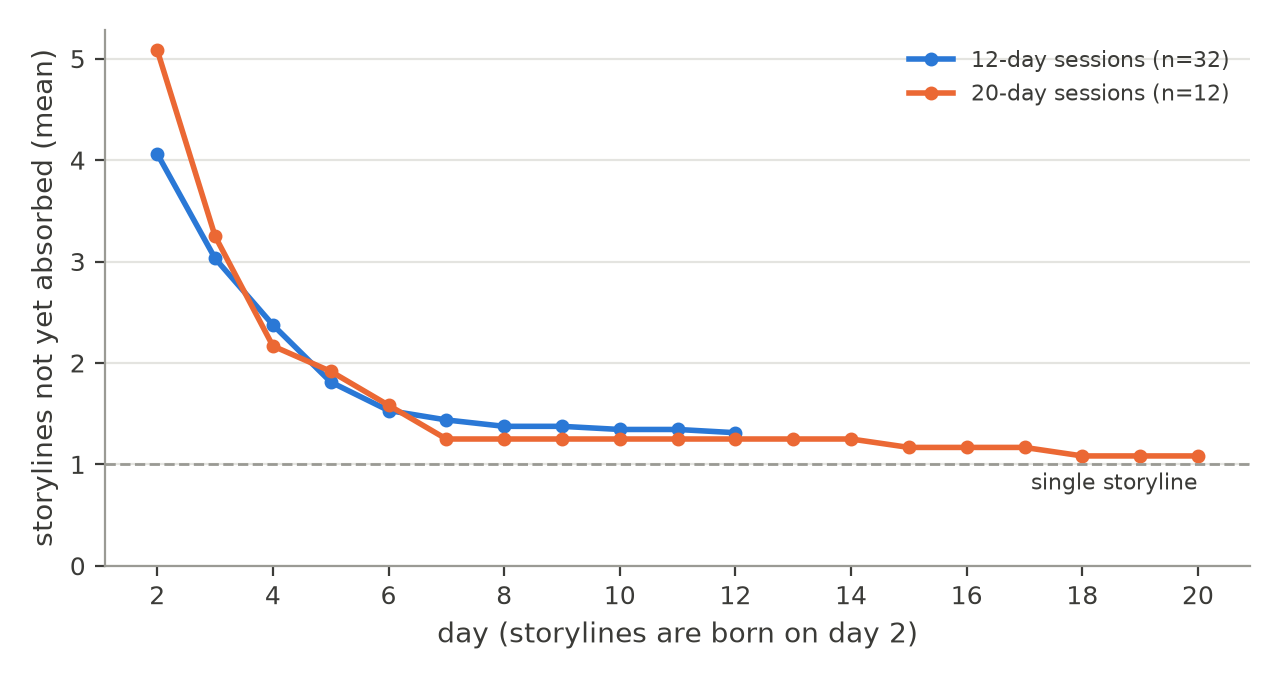
\includegraphics[width=0.78\textwidth]{bacia.png}
\caption{Storylines not yet absorbed by another storyline, mean per day.
Blue: 32 sessions of 12 days; orange: 12 sessions of 20 days.}
\label{fig:bacia}
\end{figure}

The null model shows how much of this follows from density alone. When
every event's causes are rewired at random, keeping their number, sessions
end with 1.05 storylines on average, against 1.5 observed in the first
round. In other words, the agents' links are somewhat \emph{more} local than
random links would be, and still, with almost two causes per event in a world
of six characters, everything connects. The existence of the attractor is a
consequence of linking almost every event to the past. What remains to
explain is its path: which storylines merge first, where and through what.

\subsection{Attractor events}

Most fusions are direct: in 74\% of them, the event that merges two
storylines cites causes in both. Attractor events are not hubs: incoming
links are only moderately concentrated (Gini coefficient 0.33; the top 5\%
of events receive 13\% of the links), so storylines are not pulled together
by a few central events that everything refers to.

What attractor events share is the world's premises. Of the 56 first
fusions between storylines that had not merged before, 75\% joined
characters whose premises already referred to each other, against 45\% of
all pairs of storylines in the same sessions and 61\% under the null model
(95\% interval of the null 45--76\%; one-sided $p = .036$;
Figure~\ref{fig:premissas}). The premise effect survives the discount for
density, but it is smaller than the naive comparison suggests: part of the
apparent attraction comes from the fact that well-connected characters start
larger storylines.

\begin{figure}[t]
\centering
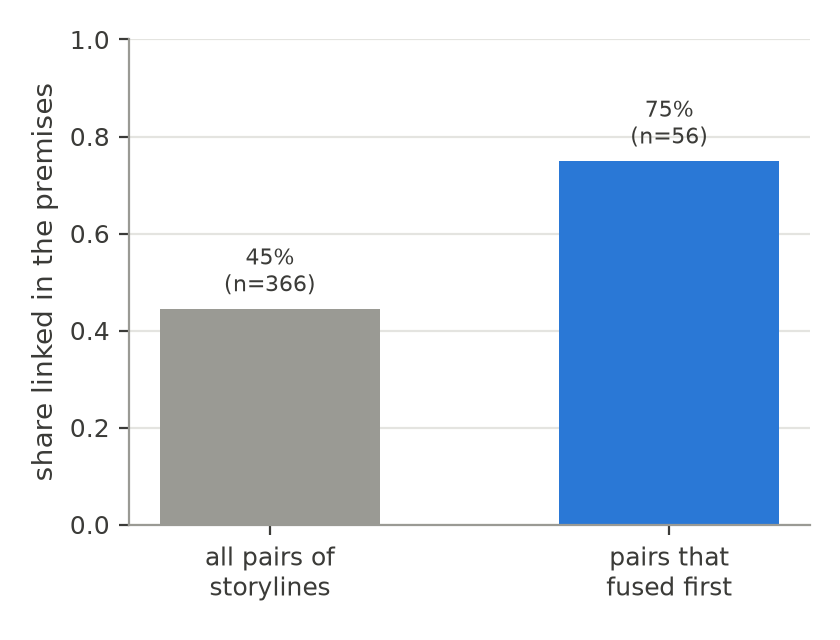
\includegraphics[width=0.48\textwidth]{premissas.png}
\caption{Share of pairs of storylines whose initiating characters are linked
in the world premises: all pairs, and the pairs that merged first.}
\label{fig:premissas}
\end{figure}

Space tells the same story (Figure~\ref{fig:lugares}). Although agents start
spread across the town, the events concentrate in the places named in more than
one premise: Vasco's warehouse and the customs house in Porto das Brumas, the
mill in Vale Silente. These places hold 49\% of all events and 57\% of the
fusion events, against 52\% under the null model (one-sided $p = .014$). The
entropy of the distribution of events over places falls from 1.96 bits in
the first two days to 1.34 bits between days 6 and 12, against a maximum of
2.32 to 2.58 bits for five or six places: the world contracts around a few
places. The objects of the premises
(the warehouse, the debt, the customs books; the mill, the stranger, the
grain) appear in 75\% of the fusion events, against 68\% of the other events
(Fisher's exact test, $p = .028$).

\begin{figure}[t]
\centering
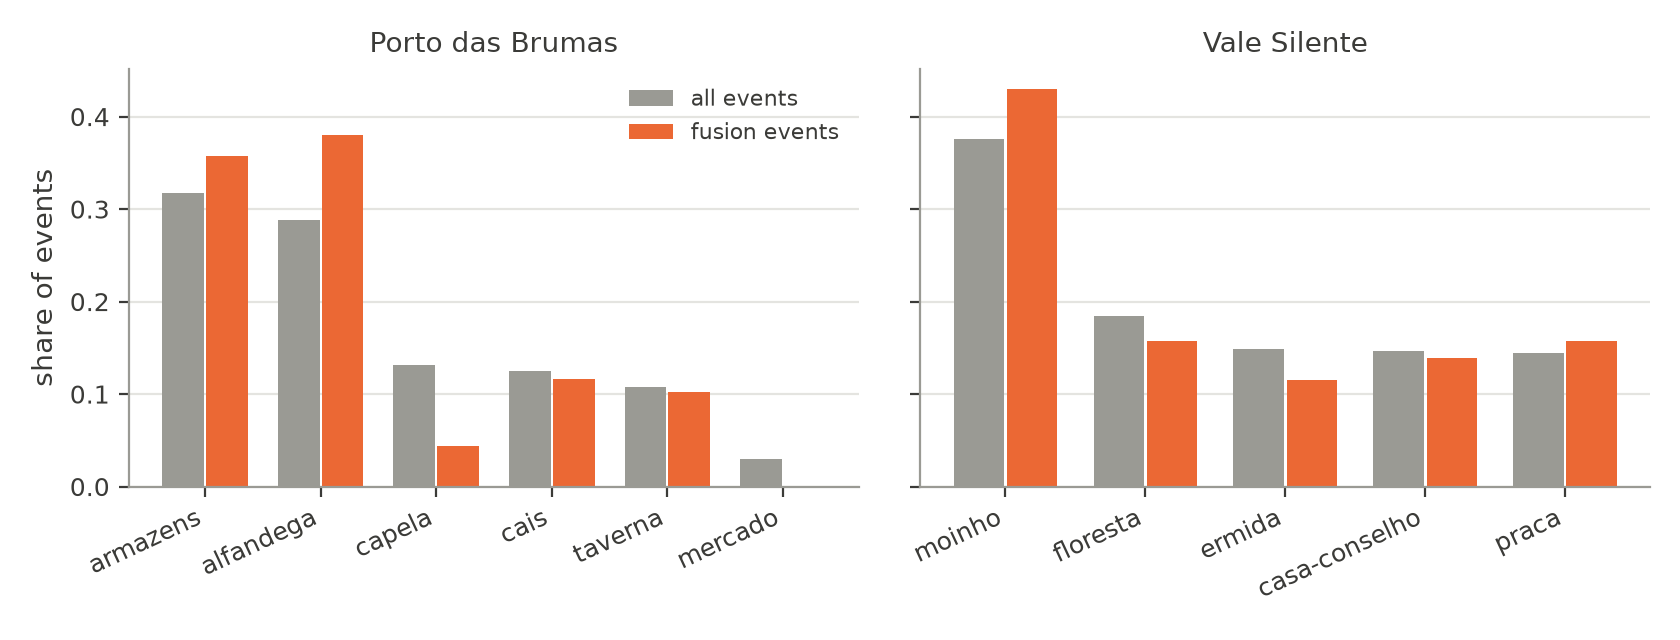
\includegraphics[width=\textwidth]{lugares.png}
\caption{Share of all events and of fusion events in each place of the two
worlds.}
\label{fig:lugares}
\end{figure}

A session of Porto das Brumas generated by \texttt{claude-opus-5}
(translated from Portuguese) shows the mechanism. On day 1, the merchant
goes to the warehouse to offer the widow a low price for it; the captain
orders the last weeks' pages of the customs books set aside \enquote{before
the new inspector reads them}; the chaplain writes down the names he saw in
the warehouse the night its owner died. Each action starts a storyline. On
day 2, in the customs house, the merchant offers the captain a purse to have
the warehouse sealed for \enquote{unpaid duties}; the captain accepts and has
the pages rewritten; the inspector asks for the books and notices the missing
pages. On day 3 the captain seals the warehouse, an action whose declared
causes are the bribe, his own acceptance and the inspector's inquiry: the
captain's and the merchant's storylines become one, in the place both of
their premises point to. The same day, the inspector goes to the warehouse
looking for the widow and finds it sealed by the captain's order. The
secrets written into the premises work as appointments: they tell the agents
where the other characters' stories are to be found.

Table~\ref{tab:resumo} summarises the measures of attraction against the
null model. The pattern is consistent: on every measure the observed
sessions deviate from random linking in the direction of the premises, and
on every measure the deviation is moderate.

\begin{table}[t]
\centering\small
\caption{Measures of attraction: observed sessions and the density-preserving
null model (500 rewirings per session; one-sided $p$ from 5,000 resamples).}
\label{tab:resumo}
\begin{tabularx}{\textwidth}{@{}Xrrr@{}}
\toprule
Measure & Observed & Null (95\% interval) & $p$ \\
\midrule
First fusions joining premise-linked characters ($n = 56$) & 75\% & 61\% (45--76\%) & .036 \\
Fusion events in places named by the premises ($n = 302$) & 57\% & 52\% (47--56\%) & .014 \\
\addlinespace
\multicolumn{4}{@{}l}{\emph{Descriptive, no null comparison}} \\
Fusions that cite causes in both storylines & 74\% & & \\
Fusion events mentioning objects of the premises & 75\% & 68\% (other events) & .028 \\
Place entropy, days 1--2 $\rightarrow$ days 6--12 (bits) & 1.96 $\rightarrow$ 1.34 & & \\
Share of links received by the top 5\% of events & 13\% & & \\
\bottomrule
\end{tabularx}
\end{table}

\subsection{Sensitivity}

Because the storyline is defined by connectivity, we repeated the lineage
analysis with alternative definitions that remove links before detection.
Removing the single links whose removal would separate two storylines of at
least three events raises the share closed by stability from 8\% to 20\%,
but does not reduce fusion (59\% to 60\%): separated storylines merge again
through other links. Cutting all links between densely connected communities
\parencite{blondel2008} gives the most permissive reading, 41\% closed and
46\% absorbed, and is best taken as an upper bound, since it also splits the
single plot of the three-act control. The direction of the result is the
same under every definition: fusion is as common as closure or more.

% ---------------------------------------------------------------------
\section{Discussion}
% ---------------------------------------------------------------------

\subsection{Two forces: density and attraction}

The convergence of these stories has two layers. The first is structural.
Language-model agents almost never act without citing something that
happened before; in a small world, a graph in which nearly every new node
links to the past becomes connected quickly, as random networks do once the
average degree passes a threshold \parencite{newman2018}. The null model
shows that density alone would merge the storylines even more completely. This
layer explains \emph{that} the story becomes one. It is a property of how
the agents relate their actions to the past, not of a particular model:
it appears with every model we tested and under every instruction we tried.

The second layer is the path. Within the time the story takes to become
one, which storylines meet, where and over what is not random. Fusions
happen when characters whose premises were written to refer to each other
meet, in the places those premises name, around the objects they mention.
These are the attractor events. Their pull is real but moderate (75\%
against 61\% expected by chance for first fusions; 57\% against 52\% for
places), which is what one would expect if the premises bias the path
without dictating it. In the language of dynamical systems, the end state is
fixed by the regime, and the premises shape the trajectory inside the
basin. The analogy with chaotic systems is apt in one more respect: two
sessions of the same world with different seeds produce different texts,
characters do different things on different days, yet the macroscopic
outcome, a single story organised around the same few places and secrets, is
the same.

This explains why interventions on the generation did not help. Asking for
typed and weighted causes made agents more explicit about connections and
therefore more connected. Asking for fewer causes changed the count, not the
choice: agents kept citing the events of other storylines that their
premises pointed to. Longer sessions only extended the time spent in the
attractor.

\subsection{What this means for AI and media literacy}

The findings matter for educational uses of generative role-play in three
ways.

\emph{First, an open world is less open than it looks.} When a teacher or a
group of students sets up a shared world and lets AI characters act, the
experience is one of freedom: nobody imposed a plot, and every session is
different. Our data show that, structurally, these sessions converge to the
same kind of story, and do so quickly. This is a structural counterpart to
the homogenisation already documented at the level of texts and plot
elements \parencite{doshi2024,xu2025}: even when no single prompt asks for a
story, the dynamics of generation pull toward one. Recognising this
convergence is part of understanding how AI shapes the content it helps
create \parencite{long2020,unesco2024}.

\emph{Second, the forces are authored, and visible.} The attractors we found
are not hidden in the model weights; they are in the premises a human wrote:
who owes whom, who knows what, where the secret is kept. This turns a
critical question about media, \enquote{who constructed this message, and
how?} \parencite{hobbs2010}, into something students can manipulate. The
same world with differently entangled premises should converge along a
different path, and the event graph makes the path visible. Tracing why two
storylines merged, and which premise brought the characters together, is
an exercise in reading how a generated narrative was constructed.

\emph{Third, the design levers are spatial and social, not textual.}
Instructions in the prompt did not change the outcome; the structure of the
world did. For designers of educational role-play this suggests acting on
the world rather than on the wording: separating characters in space,
limiting who can learn what and when, and introducing events from outside
the cast, which would be the only way to start new storylines once every
action cites the past. These are, not by coincidence, the levers of board
and tabletop game design, in which space and information channel what can
happen \parencite{jenkins2004,salen2004}. They are also levers that
students can understand without knowing anything about language models.

\subsection{A classroom protocol for critical AI literacy}

The results suggest a concrete activity, which we describe as a proposal to
be evaluated rather than as a finding. It requires only the simulator, which
runs on local open models as well as on commercial ones, and a projector.

\emph{Step 1: play.} The class designs a small world together: five or six
places, six characters, and for each character an objective, a secret and
two beliefs. Students are not told about attractors. The simulator runs for
ten in-game days, and groups follow different characters, reading the
events as a story.

\emph{Step 2: predict.} Before seeing any graph, each group writes down how
many separate stories it thinks are happening and which ones will end. In
our data, the honest answer after day five is almost always \enquote{one},
and students' predictions are a measure of how open the experience felt.

\emph{Step 3: read the graph.} The class looks at the causal graph and at
the lineage of each storyline: when it was born, which event merged it with
which other storyline, and in which place. Groups trace each fusion back to
the premises and mark the ones that were \enquote{appointments} written
into the world: two secrets about the same object, a belief about another
character, a place mentioned twice.

\emph{Step 4: intervene.} Groups rewrite the premises to move the attractors,
for example by giving two characters secrets about different places, or by
removing the object everyone wants, and run the same world again (with the
same seed, where the model accepts one). Comparing the two graphs shows what changed and what did not:
the story will probably still become one, but along a different path.

\emph{Step 5: generalise.} The discussion connects the exercise to other
generated media. A recommendation feed, a chatbot conversation or a
generated news summary also has initial conditions written by someone, and
dynamics that pull toward some outcomes more than others. The question that
media literacy asks of any message, who made it and how, becomes a question
about which premises a system was given and which attractors those
premises create.

The protocol makes three abstract ideas tangible: that generated content has
structure beyond its surface text, that the structure depends on human
design choices, and that it can be inspected. Its evaluation, with measures
of students' understanding before and after, is left for future work.

\subsection{Limitations}

All agents were models of a single family; models from other providers,
including open models run locally, are supported by the instrument and are
the obvious next step. The sessions are short and few per condition, and
they come from a validation stage: the confirmatory campaign registered in
advance has not yet been run. The storyline is defined by graph
connectivity, a standard but debatable operationalisation of
\enquote{storyline}; we reported alternative definitions for that reason. The
premise coding was done by a single coder from the world texts; a second,
independent coding is needed. The declared causes were validated by judge
models of the same family and not yet by human annotators, whose annotation
has been prepared. Finally, no learners took part in this study: the
educational implications are arguments for future classroom work, not
results.

% ---------------------------------------------------------------------
\section{Conclusion}
% ---------------------------------------------------------------------

Left to act freely in a shared world, language-model agents do not produce a
web of stories that open and close. They produce one story, quickly, because
almost every action is tied to something that already happened. Which threads
merge first, and where, is decided by attractors: the entangled premises and
the places they name, written by the humans who designed the world. For
education, the lesson is double. Generative role-play is not as open as it
feels, and the reasons are structural rather than stylistic; and the forces
that shape it are authored, legible and teachable. Making students read the
causal graph of a story they co-created with AI, and change the world to see
it converge differently, is a concrete way of practising critical AI
literacy.

\section*{Data and code availability}
The simulator, the pre-registration and its amendments, the event logs of all
sessions and the analysis scripts are available in a public repository
[link removed for review].

\printbibliography

\end{document}
